\documentclass[10pt]{article}

\usepackage{graphicx}
\usepackage{amsmath}
%\usepackage[ansinew]{inputenc}
\usepackage[utf8]{inputenc}
\usepackage[spanish]{babel}
\usepackage{babelbib}
\usepackage[T1]{fontenc}
\usepackage[vmargin=4cm,hmargin=4cm,letterpaper]{geometry}
\usepackage{color}
\usepackage{framed}
\usepackage{hyperref}

\usepackage{listings}
\definecolor{red}{RGB}{219,0,0}
\definecolor{pink}{RGB}{255,100,100}
\definecolor{gray}{RGB}{100,100,100}
\lstset{
		basicstyle=\tiny,
		frame=single,
		keywordstyle=\color{red},
		commentstyle=\color{gray},
		stringstyle=\color{pink},
		tabsize=3,
		language=verilog,
		backgroundcolor=\color{white}}

\usepackage{fancyhdr} 
\pagestyle{fancy}
\usepackage{lastpage}
\lhead{Laboratorio 3}
\chead{}
\rhead{Bitácora}
\lfoot{}
\cfoot{}
\rfoot{\footnotesize Page \thepage\ of \pageref{LastPage}}

\renewcommand{\headrulewidth}{0.4pt} 
\renewcommand{\footrulewidth}{0.4pt} 

\graphicspath{{images/}}	%%multimedia path
\setlength{\parindent}{0pt}
%%*************************************************************************
\begin{document}

\begin{huge}
\begin{center}
\textbf{Laboratorio 3: Circuitos combinatorios}
\end{center}
\end{huge}

\begin{Large}
\begin{center}
Jose Apú (B10407), Francisco Molina (B14194), \\Marco Montero (A94000), Dennis Vargas (B16831)
\end{center}
\end{Large}


\section*{Ejercicio 1}
Implemente una máquina de estados en el Spartan 6 que cumpla con la temporización necesaria para escribir y leer datos de una memoria SRAM en una plataforma Papilio Duo.\\[0.3 cm]

Para este ejercicio se instanció en la MiniAlu del Spartan 6 el controlador de una SRAM creado a partir de una máquina de estados encargada de manejar las diferentes señales necesarias en los diferentes pines para el correcto funcionamiento de la misma. Posterior a esto se escribió una serie de instrucciones en la MiniAlu de forma que la escritura y la lectura a las diferentes posiciones de la memoria fuera transparente para el usuario. Por último se escribió en la ROM un programa de prueba que escribiera y leyera datos en la memoria y escribiera los ultimos 8 bits en los LEDs de la Papilio Duo.


\begin{figure}[hbtp]
\centering
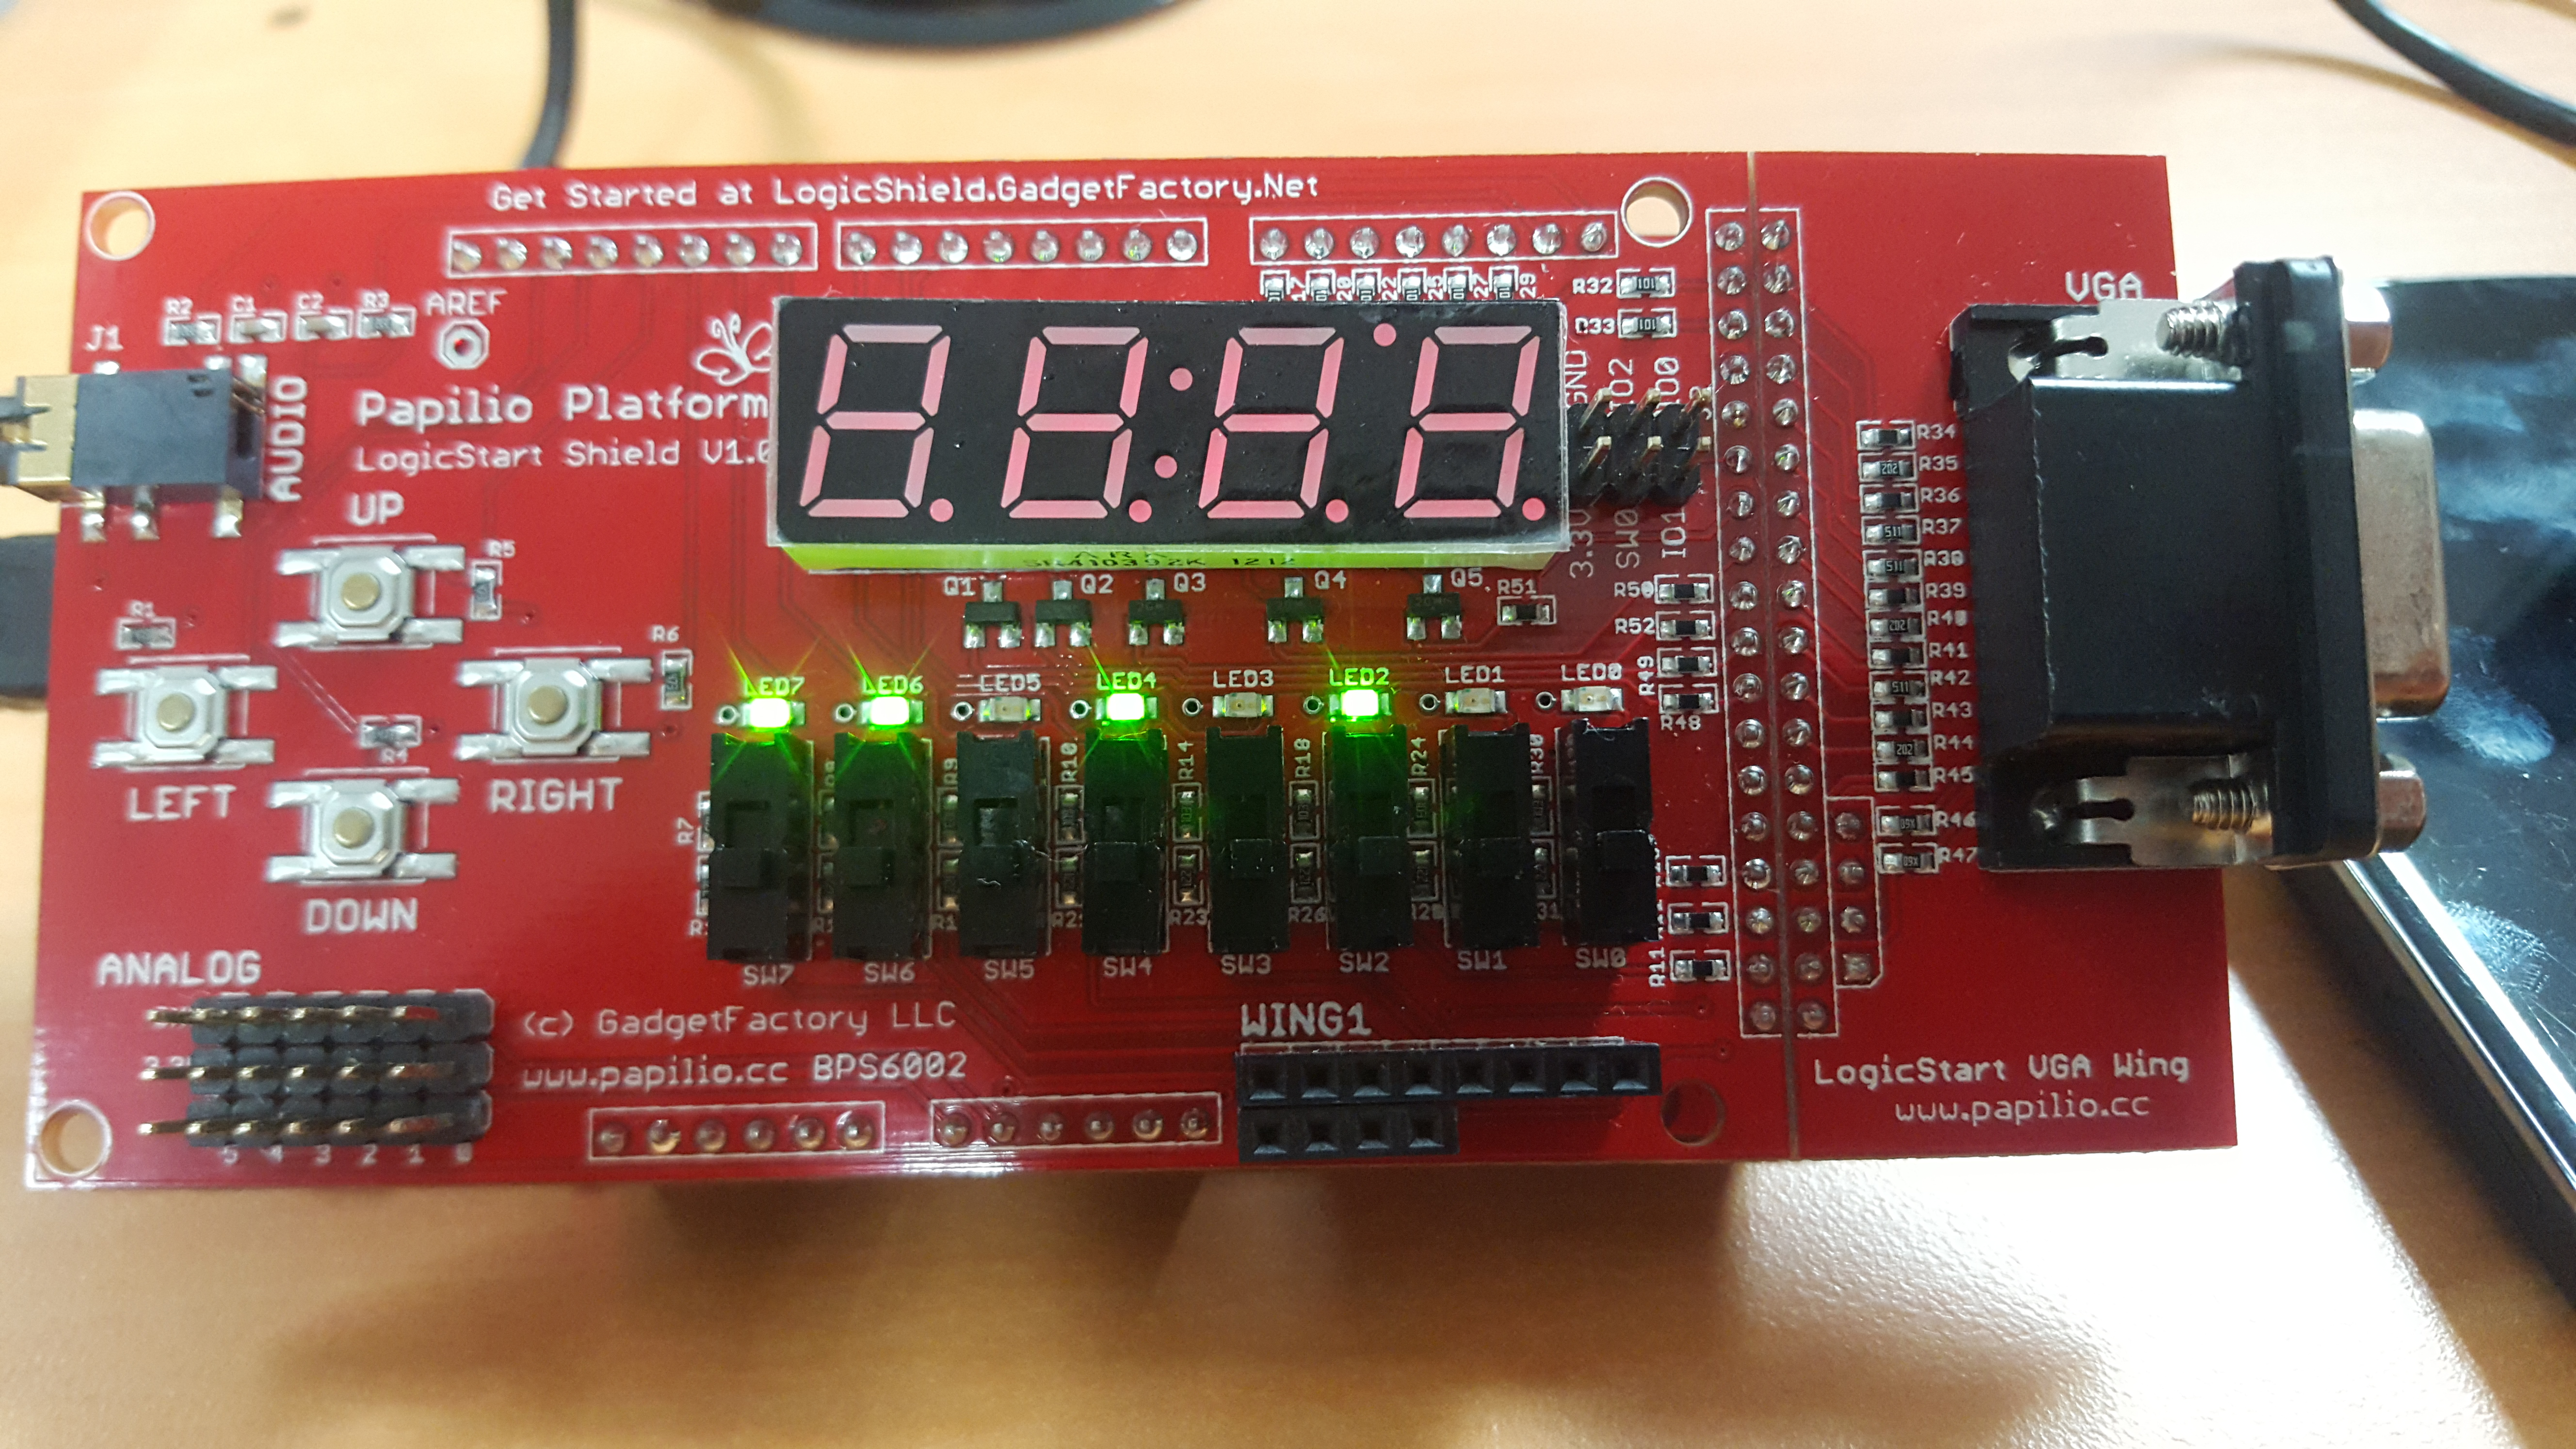
\includegraphics[width=12 cm]{read1.jpg}
\caption{Frecuencia máxima del operador * sin signo}
\label{freq1}
\end{figure}




papilio duo, tiene fpga, un wing que permite usar leds, ver que esta leyendo y escribiendo con los leds para debuggear. poner pines y comparalos con el utf.

\subsection*{SRAM controller}
\begin{lstlisting}
`define LISTEN 		  0
`define WRITE_SETUP   1
`define WRITE 		  2
`define WRITE_HOLD 	  3
`define READ_REQUEST  4
`define READ_LATCH    5


// SPARTAN 6
// CoreSpeed 32Mhz
// SRAM writting times 
// tSA  = 4ns;
// tSCE = 12ns;
// tHA  = 4ns;
// SRAM reading times
// tRC = 20ns

module SRAM_CONTROLLER # ( parameter DATA_WIDTH= 8, parameter ADDR_WIDTH=19 )
(
	input wire							Clock,
	input wire							Reset,
	
	//R/W Selection
	input wire 							iWriteEnable,	     
	//Enable the SRAM R/W
	input wire 							iTrigger,		     
	//Data from MiAlu
	input wire [ADDR_WIDTH-1:0]		iAddress,           
	//Data that the guest wants to write into SRAM
	input wire [DATA_WIDTH-1:0] 		iDataIn,            
	//Data from SRAM
	input wire [DATA_WIDTH-1:0]		iSRAMDataIn,        
	//Data that was read from SRAM
	output wire [DATA_WIDTH-1:0]		oSRAMDataRead,      
	//Data that we want to write into SRAM
	output wire [DATA_WIDTH-1:0] 		oSRAMDataWrite,     
	//Address to read/write to SRAM
	output wire [ADDR_WIDTH-1:0]		oSRAMAddressOut,     
	output reg                      oSRaMWriteEnable
);

reg wAddrEn, rDataWriteHold ;
reg rDataReadEn, rDataWriteEn;
wire [DATA_WIDTH-1:0] wSRAMDataWrite;


assign oSRAMDataWrite = ( rDataWriteEn ) ?  wSRAMDataWrite : 8'bz ;


FFD_POSEDGE_SYNCRONOUS_RESET # ( ADDR_WIDTH ) FFD_ADDR 
(
	.Clock(  Clock        ),
	.Reset(  Reset        ),
	.Enable( wAddrEn      ),
	.D(      iAddress     ),
	.Q(      oSRAMAddressOut  )
);


FFD_POSEDGE_SYNCRONOUS_RESET # ( DATA_WIDTH ) FFD_DATAOUT 
(
	.Clock(  Clock           ),
	.Reset(  Reset           ),
	.Enable( rDataWriteHold  ),
	.D(      iDataIn         ),
	.Q(      wSRAMDataWrite  )
);


FFD_POSEDGE_SYNCRONOUS_RESET # ( DATA_WIDTH ) FFD_DATAIN 
(
	.Clock(  Clock            ),
	.Reset(  Reset            ),
	.Enable( rDataReadEn      ),
	.D(      iSRAMDataIn      ),
	.Q(      oSRAMDataRead    )
);

reg [3:0] rCurrentState, rNextState;
reg [ADDR_WIDTH-1:0]    rNextAddr;
reg [DATA_WIDTH-1:0]    rNextDataOut;

//Logica de Estado Presente
always @ ( posedge Clock, posedge Reset )
begin
	if (Reset)
		rCurrentState <= `LISTEN;
	else
		rCurrentState <= rNextState;
end

//Logica de Proximo Estado de una Maquina de Mealy
always @ ( * )
begin
	case (rCurrentState)

		`LISTEN:
		begin
			//Hold address in this state to make sure it`ll be available in next state
			wAddrEn  = 1'b1;	
			rDataReadEn  = 1'b0;
			rDataWriteEn = 1'b0;
			rDataWriteHold = iWriteEnable;
			oSRaMWriteEnable = 1'b1;

			if (iTrigger)
				   rNextState = ( iWriteEnable ) ? `WRITE_SETUP : `READ_REQUEST  ;
			else 
			      rNextState = `LISTEN;
		end

		`WRITE_SETUP:
		begin
			wAddrEn          = 1'b0;
			rDataReadEn      = 1'b0;
			rDataWriteEn     = 1'b0;
			rDataWriteHold   = 1'b0;
			oSRaMWriteEnable = 1'b1;

			rNextState = `WRITE;
			
		end

		`WRITE:
		begin
			wAddrEn          = 1'b0;
			rDataReadEn      = 1'b0;
			rDataWriteEn     = 1'b0;
			rDataWriteHold   = 1'b0;
			oSRaMWriteEnable = 1'b1;

			rNextState = `WRITE_HOLD;
		end

		`WRITE_HOLD:
		begin
			wAddrEn          = 1'b0;
			rDataReadEn      = 1'b0;
			rDataWriteEn     = 1'b1;
			rDataWriteHold   = 1'b0;
			oSRaMWriteEnable = 1'b0;

			rNextState = `LISTEN;
		end

		`READ_REQUEST:			//Present address bus
		begin	
			wAddrEn          = 1'b0;
			rDataReadEn      = 1'b0;
			rDataWriteEn     = 1'b0;
			rDataWriteHold   = 1'b0;
			oSRaMWriteEnable = 1'b1;

			rNextState = `READ_LATCH;
		end

		`READ_LATCH:           //Readback data from Memory
		begin
			wAddrEn          = 1'b0;
         rDataReadEn      = 1'b1;
         rDataWriteEn     = 1'b0;
			rDataWriteHold   = 1'b0;
			oSRaMWriteEnable = 1'b1;

			rNextState = `LISTEN;
		end


		default:
		begin
			wAddrEn          =  1'b0;
			rDataReadEn      =  1'b0;
			rDataWriteEn     = 1'b0;
			rDataWriteHold   = 1'b0;
			oSRaMWriteEnable = 1'b1;

			rNextState = `LISTEN;
		end

	endcase
end

endmodule
\end{lstlisting}
Note en la figura siguiente como el simulador reconoce la multiplicación con signo:

%%**********************************************************************
\section{Prueba}
Primero se escriben los datos en la SRAM. Para lograrlo, se escribe en la ROM lo siguiente:

\begin{lstlisting}
...
4: oInstruction = { `STO , `R4, 8'b0, 8'b11010100};
5: oInstruction = { `STO , `R5, 8'b0, 8'b11101000};
...
7: oInstruction = { `SWR , 8'hff, `R4, `R1};
...
11: oInstruction = { `SWR , 8'hff, `R5, `R2};
...
\end{lstlisting}

En la simulación se observa como se escriben los datos escritos, ver Figura \ref{sim_escritura}

% Adding an image
\begin{figure}[hbtp]
\centering
\includegraphics[width=1\textwidth]{escritura.png}
\caption{Simulación: Escritura}
\label{sim_escritura}
\end{figure}

Para leerlos se utilizan los leds. Para lograrlo, se escribe en la ROM lo siguiente:

\begin{lstlisting}
...
17: oInstruction = { `SRD , `R4, 8'hff, `R1};
...
21: oInstruction = { `LED , 8'hff, 8'hff, `R4 };
...
28: oInstruction = { `SRD , `R5, 8'hff, `R2};
...
32: oInstruction = { `LED , 8'hff, 8'hff, `R5 };
...
\end{lstlisting}

En las fotografías se observan como los leds ilustran los dos datos escritos y a su vez leidos. Ver Figuras \ref{lectura_1} y \ref{lectura_2}

% Adding an image
\begin{figure}[hbtp]
\centering
\includegraphics[width=1\textwidth]{lecturaa.jpg}
\caption{Lectura del primer dato}
\label{lectura_1}
\end{figure}

% Adding an image
\begin{figure}[hbtp]
\centering
\includegraphics[width=1\textwidth]{lecturab.jpg}
\caption{Lectura del segundo dato}
\label{lectura_2}
\end{figure}
\pagebreak
%%**********************************************************************
\section{Conlusiones}
Se logra determinar q apartir de maquinas de estado es posible obtener un mecanismo de lectura y escritura.\\
Con la ayuda del diagrama de pin-out de la tarjeta papilio, fue posible comunicar la spartan6 con la SRAM.\\
%%**********************************************************************
\section{Bibliografía}
\begin{itemize}
\item Bib1
\end{itemize}

\end{document}
%%*************************************************************************
